% Options for packages loaded elsewhere
\PassOptionsToPackage{unicode}{hyperref}
\PassOptionsToPackage{hyphens}{url}
%
\documentclass[
]{article}
\usepackage{amsmath,amssymb}
\usepackage{lmodern}
\usepackage{iftex}
\ifPDFTeX
  \usepackage[T1]{fontenc}
  \usepackage[utf8]{inputenc}
  \usepackage{textcomp} % provide euro and other symbols
\else % if luatex or xetex
  \usepackage{unicode-math}
  \defaultfontfeatures{Scale=MatchLowercase}
  \defaultfontfeatures[\rmfamily]{Ligatures=TeX,Scale=1}
\fi
% Use upquote if available, for straight quotes in verbatim environments
\IfFileExists{upquote.sty}{\usepackage{upquote}}{}
\IfFileExists{microtype.sty}{% use microtype if available
  \usepackage[]{microtype}
  \UseMicrotypeSet[protrusion]{basicmath} % disable protrusion for tt fonts
}{}
\makeatletter
\@ifundefined{KOMAClassName}{% if non-KOMA class
  \IfFileExists{parskip.sty}{%
    \usepackage{parskip}
  }{% else
    \setlength{\parindent}{0pt}
    \setlength{\parskip}{6pt plus 2pt minus 1pt}}
}{% if KOMA class
  \KOMAoptions{parskip=half}}
\makeatother
\usepackage{xcolor}
\usepackage[margin=1in]{geometry}
\usepackage{color}
\usepackage{fancyvrb}
\newcommand{\VerbBar}{|}
\newcommand{\VERB}{\Verb[commandchars=\\\{\}]}
\DefineVerbatimEnvironment{Highlighting}{Verbatim}{commandchars=\\\{\}}
% Add ',fontsize=\small' for more characters per line
\usepackage{framed}
\definecolor{shadecolor}{RGB}{248,248,248}
\newenvironment{Shaded}{\begin{snugshade}}{\end{snugshade}}
\newcommand{\AlertTok}[1]{\textcolor[rgb]{0.94,0.16,0.16}{#1}}
\newcommand{\AnnotationTok}[1]{\textcolor[rgb]{0.56,0.35,0.01}{\textbf{\textit{#1}}}}
\newcommand{\AttributeTok}[1]{\textcolor[rgb]{0.77,0.63,0.00}{#1}}
\newcommand{\BaseNTok}[1]{\textcolor[rgb]{0.00,0.00,0.81}{#1}}
\newcommand{\BuiltInTok}[1]{#1}
\newcommand{\CharTok}[1]{\textcolor[rgb]{0.31,0.60,0.02}{#1}}
\newcommand{\CommentTok}[1]{\textcolor[rgb]{0.56,0.35,0.01}{\textit{#1}}}
\newcommand{\CommentVarTok}[1]{\textcolor[rgb]{0.56,0.35,0.01}{\textbf{\textit{#1}}}}
\newcommand{\ConstantTok}[1]{\textcolor[rgb]{0.00,0.00,0.00}{#1}}
\newcommand{\ControlFlowTok}[1]{\textcolor[rgb]{0.13,0.29,0.53}{\textbf{#1}}}
\newcommand{\DataTypeTok}[1]{\textcolor[rgb]{0.13,0.29,0.53}{#1}}
\newcommand{\DecValTok}[1]{\textcolor[rgb]{0.00,0.00,0.81}{#1}}
\newcommand{\DocumentationTok}[1]{\textcolor[rgb]{0.56,0.35,0.01}{\textbf{\textit{#1}}}}
\newcommand{\ErrorTok}[1]{\textcolor[rgb]{0.64,0.00,0.00}{\textbf{#1}}}
\newcommand{\ExtensionTok}[1]{#1}
\newcommand{\FloatTok}[1]{\textcolor[rgb]{0.00,0.00,0.81}{#1}}
\newcommand{\FunctionTok}[1]{\textcolor[rgb]{0.00,0.00,0.00}{#1}}
\newcommand{\ImportTok}[1]{#1}
\newcommand{\InformationTok}[1]{\textcolor[rgb]{0.56,0.35,0.01}{\textbf{\textit{#1}}}}
\newcommand{\KeywordTok}[1]{\textcolor[rgb]{0.13,0.29,0.53}{\textbf{#1}}}
\newcommand{\NormalTok}[1]{#1}
\newcommand{\OperatorTok}[1]{\textcolor[rgb]{0.81,0.36,0.00}{\textbf{#1}}}
\newcommand{\OtherTok}[1]{\textcolor[rgb]{0.56,0.35,0.01}{#1}}
\newcommand{\PreprocessorTok}[1]{\textcolor[rgb]{0.56,0.35,0.01}{\textit{#1}}}
\newcommand{\RegionMarkerTok}[1]{#1}
\newcommand{\SpecialCharTok}[1]{\textcolor[rgb]{0.00,0.00,0.00}{#1}}
\newcommand{\SpecialStringTok}[1]{\textcolor[rgb]{0.31,0.60,0.02}{#1}}
\newcommand{\StringTok}[1]{\textcolor[rgb]{0.31,0.60,0.02}{#1}}
\newcommand{\VariableTok}[1]{\textcolor[rgb]{0.00,0.00,0.00}{#1}}
\newcommand{\VerbatimStringTok}[1]{\textcolor[rgb]{0.31,0.60,0.02}{#1}}
\newcommand{\WarningTok}[1]{\textcolor[rgb]{0.56,0.35,0.01}{\textbf{\textit{#1}}}}
\usepackage{graphicx}
\makeatletter
\def\maxwidth{\ifdim\Gin@nat@width>\linewidth\linewidth\else\Gin@nat@width\fi}
\def\maxheight{\ifdim\Gin@nat@height>\textheight\textheight\else\Gin@nat@height\fi}
\makeatother
% Scale images if necessary, so that they will not overflow the page
% margins by default, and it is still possible to overwrite the defaults
% using explicit options in \includegraphics[width, height, ...]{}
\setkeys{Gin}{width=\maxwidth,height=\maxheight,keepaspectratio}
% Set default figure placement to htbp
\makeatletter
\def\fps@figure{htbp}
\makeatother
\setlength{\emergencystretch}{3em} % prevent overfull lines
\providecommand{\tightlist}{%
  \setlength{\itemsep}{0pt}\setlength{\parskip}{0pt}}
\setcounter{secnumdepth}{-\maxdimen} % remove section numbering
\ifLuaTeX
  \usepackage{selnolig}  % disable illegal ligatures
\fi
\IfFileExists{bookmark.sty}{\usepackage{bookmark}}{\usepackage{hyperref}}
\IfFileExists{xurl.sty}{\usepackage{xurl}}{} % add URL line breaks if available
\urlstyle{same} % disable monospaced font for URLs
\hypersetup{
  pdftitle={Installing R and RStudio},
  pdfauthor={Rob Cavanaugh},
  hidelinks,
  pdfcreator={LaTeX via pandoc}}

\title{Installing R and RStudio}
\author{Rob Cavanaugh}
\date{2022-08-07}

\begin{document}
\maketitle

\hypertarget{objectives}{%
\section{Objectives:}\label{objectives}}

\begin{itemize}
\tightlist
\item[$\square$]
  Install R
\item[$\square$]
  Install Rstudio
\item[$\square$]
  Install some R packages
\end{itemize}

\hypertarget{what-is-r-and-why-use-it}{%
\section{What is R, and why use it?}\label{what-is-r-and-why-use-it}}

R is a \emph{free} programming environment for data processing and
statistical analysis. R allows you to write scripts that combine data
files, clean data, and run analyses. R is really useful for conducting
reproducible research (research that documents all of the steps between
raw data and results in a way that can be verified), automating
analytical steps, creating custom high-quality visualizations, and
conducting a wide range of statistical analyses from basic t-tests to
multivariate multilevel Bayesian regression.

This document details steps to get started in R as part of the R for
researchers in Communication Sciences and Disorders workshop (August
2022). It synthesizes already-published materials for teaching R in a
way that is tailored to this workshop. Anyone interested in the full
materials can find them here: \url{https://psyteachr.github.io/}.

\hypertarget{installing-r}{%
\section{Installing R}\label{installing-r}}

\emph{note, more detailed instructions can be found here:
\url{https://rstudio-education.github.io/hopr/starting.html}}

\href{https://cran.rstudio.com/}{Install base R}. This installs the R
programming language and a simple GUI (from here on, we will refer to it
as the R GUI). Choose the download link for your operating system
(Linux, Mac OS X, or Windows).

\begin{figure}
\centering
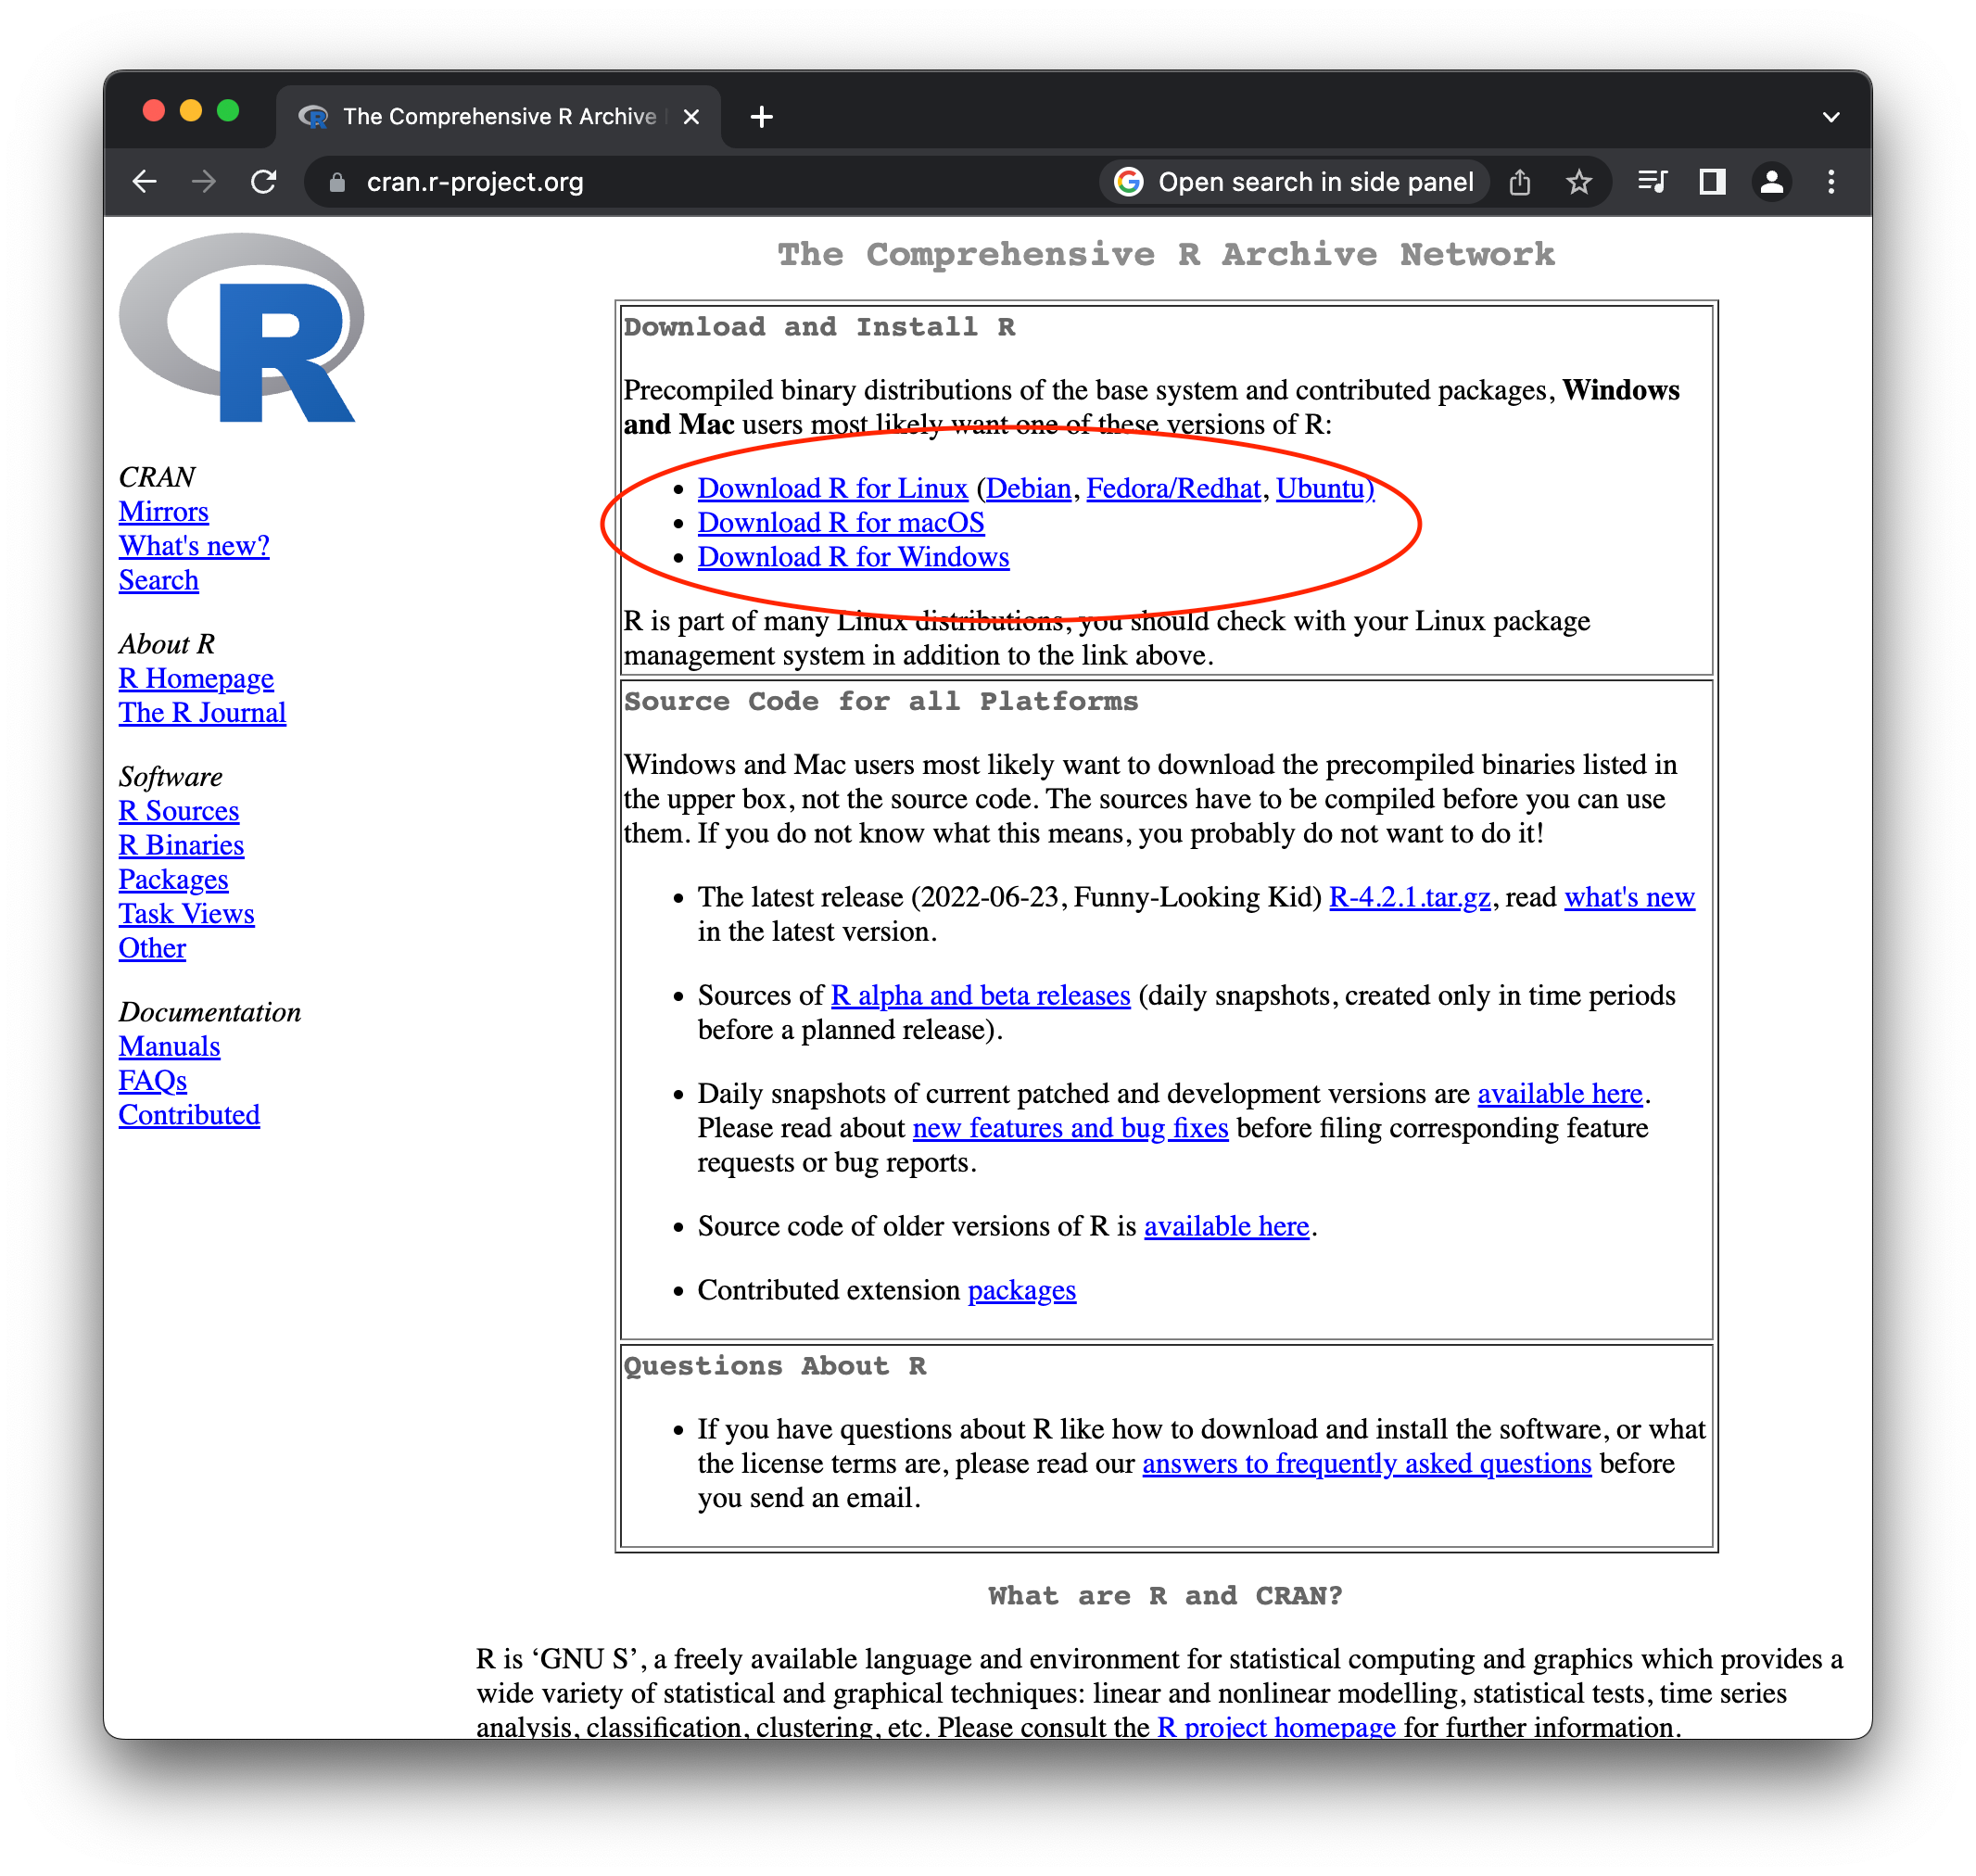
\includegraphics[width=4.16667in,height=\textheight]{images/paste-B40FB4F4.png}
\caption{Download page for R and the R GUI}
\end{figure}

If you have a \textbf{Mac}, install the latest release from the newest
\texttt{R-x.x.x.pkg} link (or a legacy version if you have an older
operating system). After you install R, you should also install
\href{http://xquartz.macosforge.org/}{XQuartz} to be able to use some
visualisation packages.

If you are installing the \textbf{Windows} version, choose the
``\href{https://cran.rstudio.com/bin/windows/base/}{base}'' subdirectory
and click on the download link at the top of the page. After you install
R, you should also install
\href{https://cran.rstudio.com/bin/windows/Rtools/}{RTools}; use the
``recommended'' version highlighted near the top of the list.

If you are using \textbf{Linux}, choose your specific operating system
and follow the installation instructions.

If you have trouble with installation, R can also be used online:
\href{https://rstudio.cloud/}{RStudio Cloud} is a free online service
that allows access to R and RStudio.

\begin{figure}
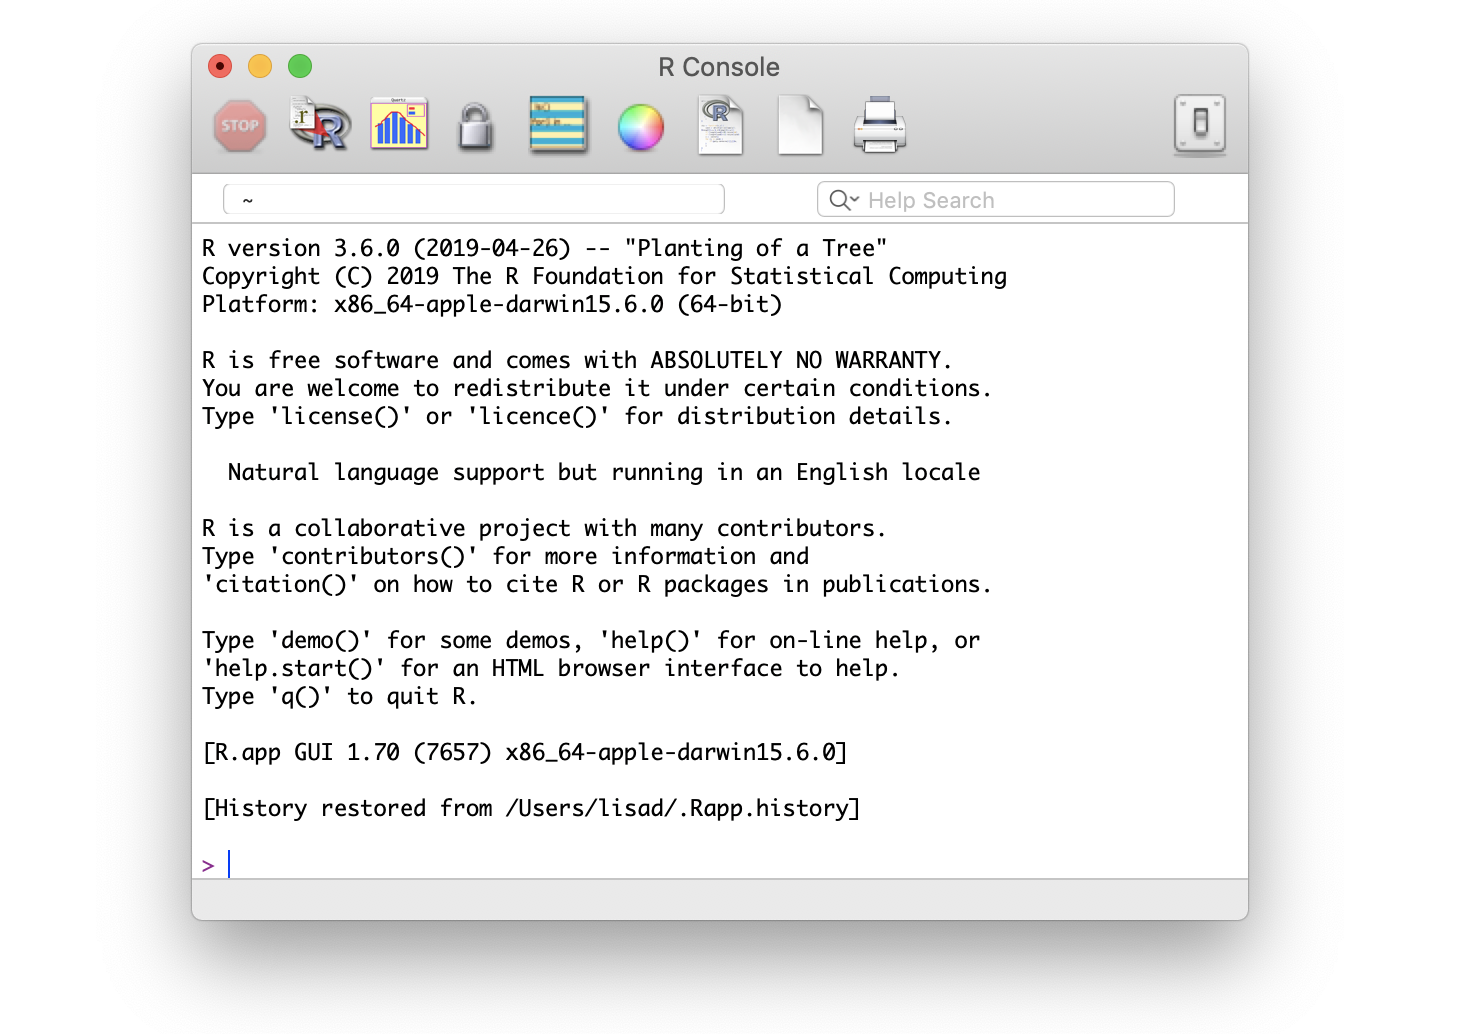
\includegraphics[width=400px]{images/paste-8DC0F4C7} \caption{A view of the R GUI on mac}\label{fig:unnamed-chunk-1}
\end{figure}

\hypertarget{installing-rstudio}{%
\section{Installing RStudio}\label{installing-rstudio}}

RStudio is an ``IDE'' (Integrated Development Environment) for using R
(and some other languages). RStudio allows us to run R code and comes
with lots of other features that makes using R easier and more
efficient.

Go to
\href{https://www.rstudio.com/products/rstudio/download/\#download}{rstudio.com}
and download the RStudio Desktop (Open Source License) version for your
operating system under the list titled \textbf{Installers for Supported
Platforms}.

If you're unsure about where something is in RStudio, try finding it in
the cheat sheet here:
\url{https://raw.githubusercontent.com/rstudio/cheatsheets/main/rstudio-ide.pdf}

\begin{figure}
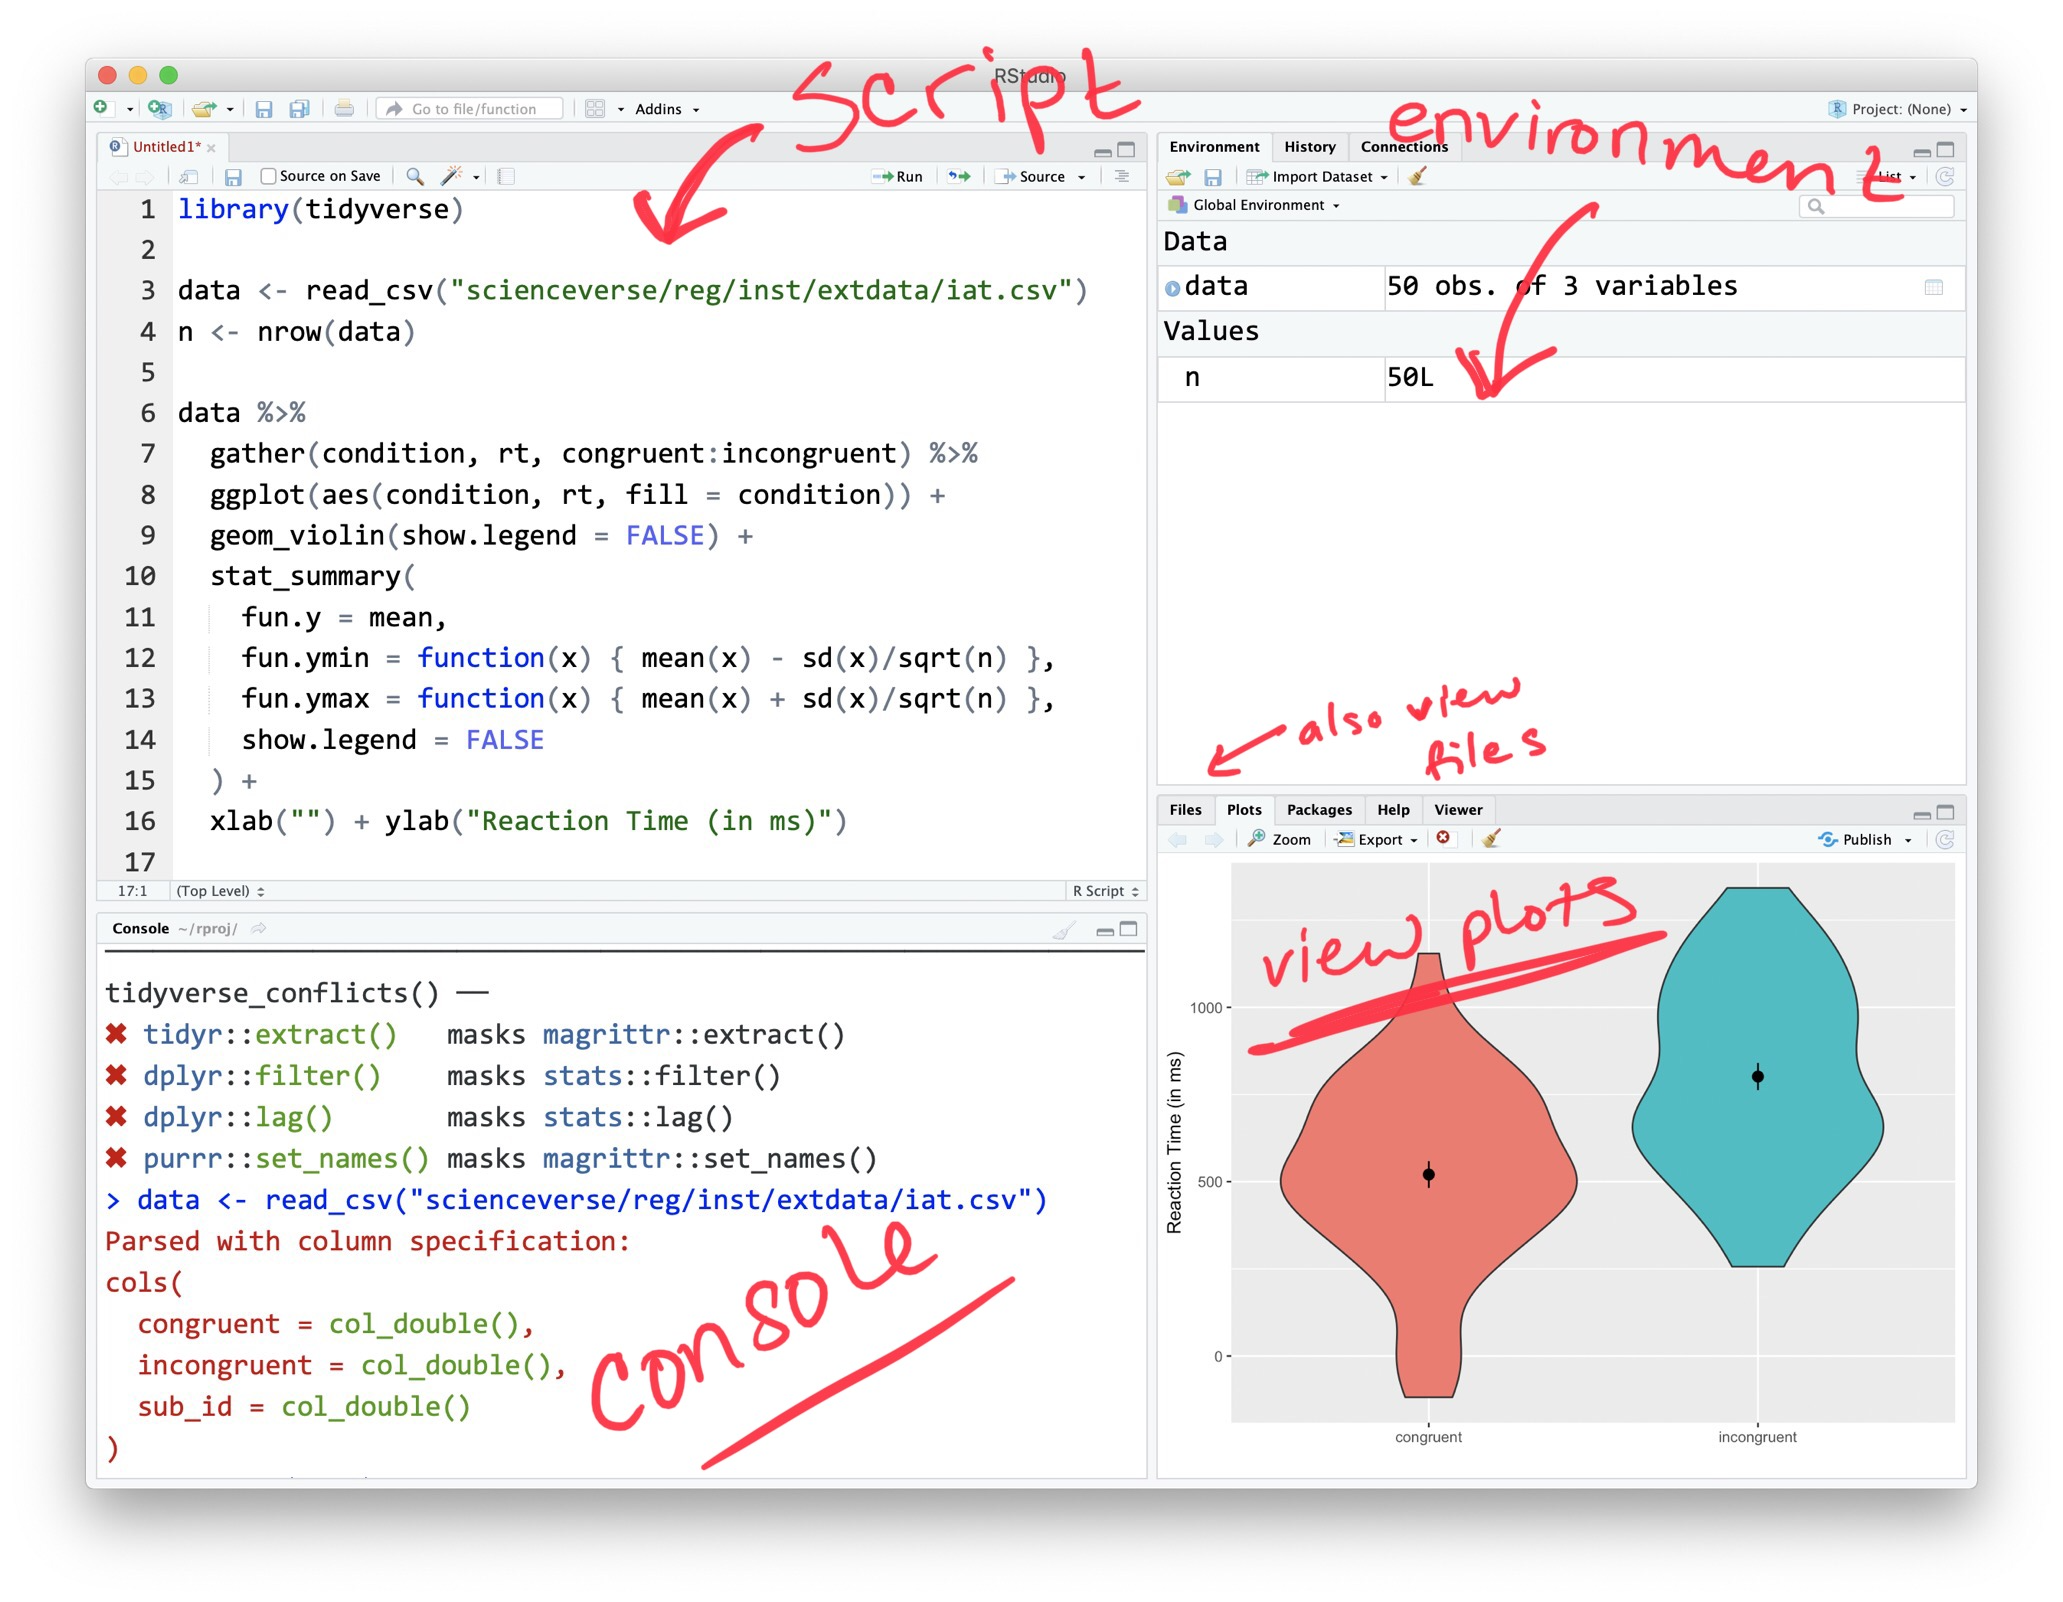
\includegraphics[width=500px]{images/paste-B4148C41} \caption{The RStudio interface}\label{fig:unnamed-chunk-2}
\end{figure}

There are a few settings you should fix immediately after updating
RStudio. Go to \textbf{\texttt{Global\ Options...}} under the
\textbf{\texttt{Tools}} menu (⌘,), and in the General tab, uncheck the
box that says
\textbf{\texttt{Restore\ .RData\ into\ workspace\ at\ startup}}. If you
keep things around in your workspace, things will get messy, and
unexpected things will happen. You should always start with a clear
workspace. This also means that you never want to save your workspace
when you exit, so set this to \textbf{\texttt{Never}}. The only thing
you want to save are your scripts.

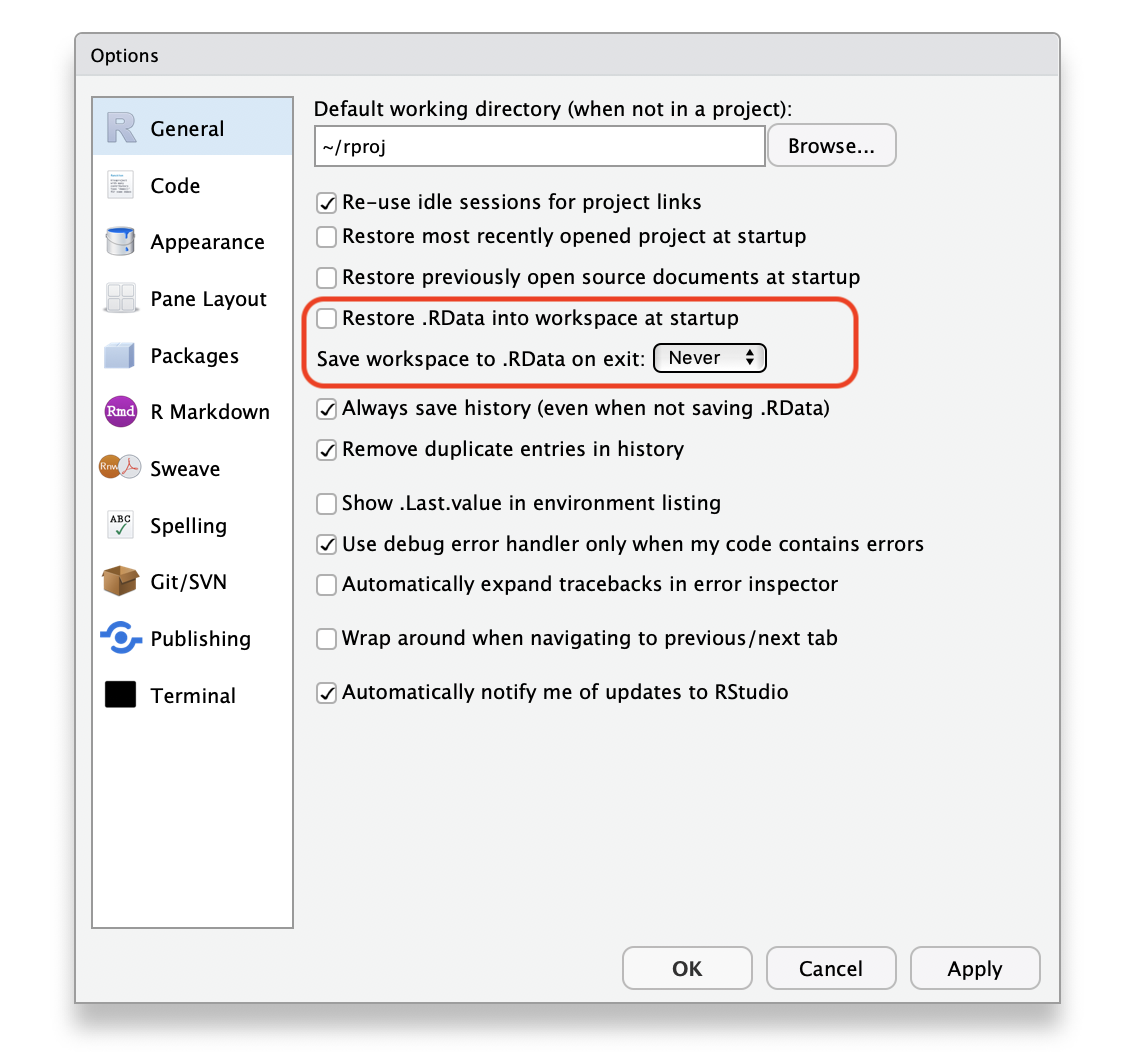
\includegraphics[width=500px]{images/paste-EA4637C3}

\emph{If you're having trouble finding this setting, make a note to
yourself and let us know when we get started on day 1}

\hypertarget{installing-packages}{%
\section{Installing Packages}\label{installing-packages}}

``base R'' (everything that comes with the initial installation of R)
comes with many basic functions for data wrangling, plotting, and
statistical analysis, but most people (including us, and this workshop)
use additional packages that add additional features to R.

The main repository where packages reside is called
\href{https://psyteachr.github.io/glossary/c\#cran}{CRAN}, the
Comprehensive R Archive Network. A package has to pass strict tests
devised by the R core team to be allowed to be part of the CRAN archive.
You can install from the CRAN archive with the
\href{https://rdrr.io/r/utils/install.packages.html}{\texttt{install.packages}}\texttt{()}
function. Try installing the following packages:

\begin{Shaded}
\begin{Highlighting}[]
\CommentTok{\# installs the package tidyverse, which includes data wrangling and viz tools}
\FunctionTok{install.packages}\NormalTok{(}\StringTok{"tidyverse"}\NormalTok{)}
\CommentTok{\# installs the package here, which helps with file management}
\FunctionTok{install.packages}\NormalTok{(}\StringTok{"here"}\NormalTok{)}
\CommentTok{\# install the usethis package, which has lots of useful functions}
\FunctionTok{install.packages}\NormalTok{(}\StringTok{"usethis"}\NormalTok{)}
\end{Highlighting}
\end{Shaded}

Sometimes, installing packages can result in errors. If you run into an
error, copy and paste the error into a sticky/note on your computer and
save it for the beginning of the workshop.

\emph{Note: Never install packages within a script, only install scripts
from the console}

\hypertarget{installing-latex-optional}{%
\section{Installing LaTeX (optional)}\label{installing-latex-optional}}

You can install the LaTeX typesetting system to produce PDF reports from
RStudio. To generate PDF reports, you will additionally need to install
\textbf{\texttt{tinytex}}
(\href{https://psyteachr.github.io/reprores-v2/bookrefs.html\#ref-R-tinytex}{Xie,
2022}) package and run the following code:

\begin{Shaded}
\begin{Highlighting}[]
\FunctionTok{install.packages}\NormalTok{(}\StringTok{"tinytex"}\NormalTok{)}
\NormalTok{tinytex}\SpecialCharTok{::}\FunctionTok{install\_tinytex}\NormalTok{()}
\end{Highlighting}
\end{Shaded}

\hypertarget{troubleshooting}{%
\section{Troubleshooting}\label{troubleshooting}}

Occasionally, you might have a few problem packages that don't install
or update cleanly. If you try to update a package and get an error
message that says something like \emph{Warning in install.packages :
installation of package `vctrs' had non-zero exit status} or perhaps
\emph{Error in loadNamespace(i, c(lib.loc, .libPaths()), versionCheck =
vI{[}{[}i{]}{]}) : namespace `rlang' 0.4.9 is being loaded, but
\textgreater= 0.4.10 is required}. One solution I have found is to
manually uninstall the package, restart R, and then install the package
new, rather than trying to update an existing version.

\begin{Shaded}
\begin{Highlighting}[]
\CommentTok{\# Uninstall the problem package}
\FunctionTok{remove.packages}\NormalTok{(}\StringTok{"package\_name"}\NormalTok{)}

\CommentTok{\# Then restart R. Choose session from the top menu and then restart R}

\CommentTok{\# Then install the package fresh}
\FunctionTok{install.packages}\NormalTok{(}\StringTok{"package"}\NormalTok{)}
\end{Highlighting}
\end{Shaded}


\end{document}
